\documentclass[a4paper]{article}

\usepackage[utf8]{inputenc}
\usepackage[spanish]{babel}
\usepackage[pdftex]{color,graphicx}
\usepackage{caption}

\usepackage[pdftex,
	colorlinks=true,
	pdfauthor={Alejandro Vicario Espinosa},
	pdftitle={}]{hyperref}

\graphicspath{ {curvas/} }

\begin{document}

\title{Entregable 2 \\
\large RealLabo 2018. Modelado e implementación}
\author{
	Juan José Alberca\\
	\texttt{jj.alberca@alumnos.upm.es}
	\and
	Alejandro Vicario\\
	\texttt{a.vicarioe@alumnos.upm.es}
}
\date{\today}


\maketitle


\section{Diseño e implementación de arquitectura software en el hardware del RealLabo}
\subsection{Hardware}

\subsubsection{Conexionado}
Se ha procurado hacer el conexionado lo más simple posible, intentando respetar lo máximo posible las conexiones que ya proporciona la \emph{shield} del puente en H.
Las únicas conexiones externas a la placa que se han realizado son las que provienen del motor, que son las siguientes:
la alimentación del motor no se ha cambiado y se encuentra en el canal 1 del puente en H;
la alimentación del encoder se ha conectado a alguna de las salidas de \emph{3.3V} y \emph{GND} de la placa;
los cables amarillo y blanco del encoder se han conectado en los pines \texttt{A8} y \texttt{A9} de la placa respectivamente.

\subsubsection{Obtención de PWM}
En esta sección se pretende explicar el procedimiento seguido para obtener la señal modulada en ancho de pulso (\emph{PWM}) para controlar la potencia entregada al motor.

El microprocesador cuenta con ocho periféricos \emph{PWM}, cuya única función es generar señales de este tipo. Sin embargo,
las salidas de estos periféricos son fijas y además no coinciden con los pines que se necesitan para controlar el puente en H, 4 y 5, en la placa del Arduino,
lo cual nos obligaría a utilizar un cable adicional para poder usar este periférico. Esta información se ha encontrado en el apartado 38 del datasheet \cite{SAM3X/A}.

La placa también cuenta con timers los cuales pueden trabajar en modo \emph{waveform}.
Este modo permite generar una señal de diferentes características.
Configurando estos periféricos correctamente se puede generar una señal \emph{PWM} justo en el pin donde se conecta una de las entradas del puente en H: el pin 5.
Para generar esta señal se utilizó el canal 0 del \emph{timer} 2 (\texttt{TIOA6}), que coincide con la entrada \texttt{IN\_2} del puente en H. Para saber cómo configurar esto
se ha seguido la información hallada en el apartado 36 del datasheet \cite{SAM3X/A}.

\subsubsection{Quadrature decoder}
El \textbf{SAM3XE8} contiene un decodificador de las señales del encoder del motor en hardware,
que permite controlar su posición y/o su velocidad sin ningún software adicional, usando los canales 0, 1 y 2 del \emph{timer} 0 (\texttt{TC0}) para este propósito.
Sin embargo, no es fácil de integrar en este proyecto, ya que la entrada de \emph{Enable} del canal 1 del puente H, coincide con una de las entradas del decodificador (\emph{TIOA0}).
Por lo que habría que modificar la \emph{shield} para dejar las entradas \texttt{TIOA0} y \texttt{TIOB0} libres. La información sobre \emph{Quadrature decoder} se encuentra en el apartado
36.6.14 del datasheet \cite{SAM3X/A}.

Por lo tanto la lectura de la posición del motor se realiza mediante interrupciones y rutinas software.

\subsubsection{Interrupciones \label{int}}
Se ha activado una interrupción periódica del \emph{SysTick} cada milisegundo para obtener un contador fiable del tiempo transcurrido.
Se ha utilizado también otra interrupción periódica a un milisegundo usando el canal 1 del \emph{timer} 0 para realizar diversas tareas en software que requieren temporización.

Por último también se ha activado una interrupción por flanco de subida o bajada en los pines de entrada a los que está conectado el encoder para realizar la decodificación de la posición.

\subsection{Software \label{sec:software}}
El software utilizado se ha desarrollado sobre el \emph{framework} \cite{framework} que Atmel proporciona para sus dispositivos: \textbf{Atmel Software Framework}.
Todo el código se encuentra en un repositorio de GitHub \cite{git}.

Del software cabe destacar que se ha intentado realizar la mayoría de las tareas utilizando los periféricos hardware. Por lo tanto,
la mayor parte del código consiste en drivers que sirven para inicializar estos periféricos e interactuar con las funciones de los mismos.

Para controlar el sistema se ha implementado una interfaz de comunicación con el sistema mediante el puerto serie con el objetivo de fácilitar su uso.
Cuenta con un control de velocidad manual, con una rutina que realiza los test que se necesitan para obtener los datos utilizados para el modelado del motor y los vuelca
por el puerto serie para que puedan ser almacenados en un fichero y un control de la posición para demostrar lo mostrado en el apartado \ref{control}.

\section{Modelado experimental de un motor DC con la arquitectura hardware y software implementadas}
\subsection{Experimentos realizados \label{sec:exp}}
A partir del software descrito en la sección \ref{sec:software} se han realizado test para obtener la de respuesta al escalón del motor,
tanto para condiciones iniciales nulas y no nulas.
Para esto se ha excitado el motor con una señal cuadrada que introduce un voltaje durante $600ms$ e introduce $0V$ por otros $600ms$
mientras se toman valores de los pulsos capturados por el encoder cada milisegundo.

Esta prueba se ha repetido 10 veces para cada uno de los siguiente valores eficaces de la señal de excitación:

\begin{displaymath}
V \in \{1,2,3,4,5,6,7,8,9,10,11,12\}
\end{displaymath}

Es decir, se tienen $P=10$ repeticiones de $Q=12$ experimentos. El eje del motor tiene, por su parte, una q=48 pulsos/vuelta.
El procedimiento seguido es el explicado en la sección 3.2 del documento modelado de la asignatura \cite{modelado}.

Se han promediado las P repeticiones en cada uno de los experimentos y con ello se obtienen los datos de la figura \ref{datos} que los \emph{scripts}
de Matlab proporcionados usan en sus cálculos para modelar el motor.


\begin{figure}[hbp]
	\begin{center}
		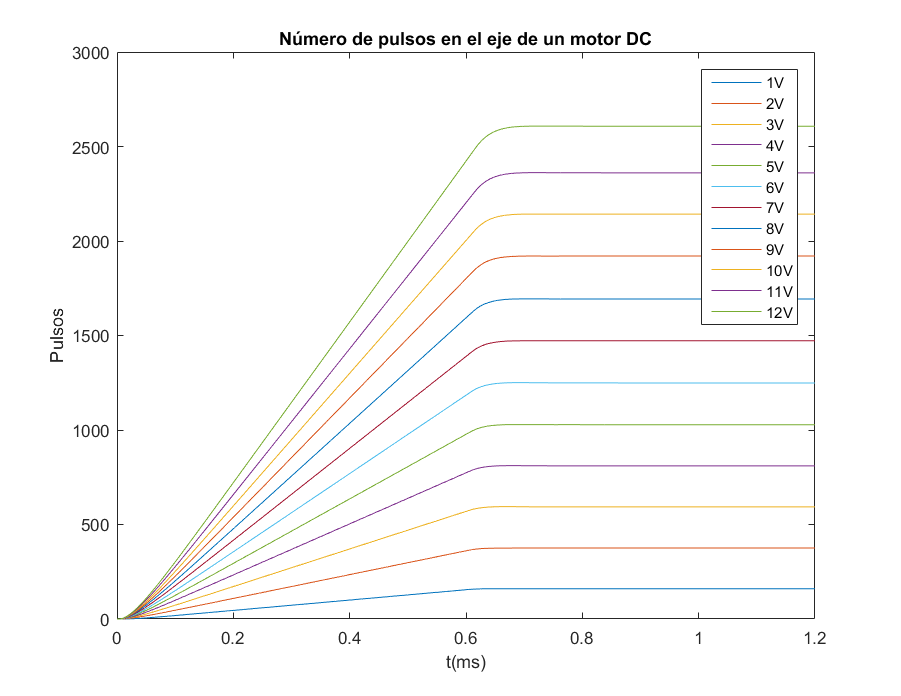
\includegraphics[width=8cm]{n_pulsos}
		\caption{Media de los datos obtenidos del motor DC.}
		\label{datos}
	\end{center}
\end{figure}

\subsection{Obtención de la función de transferencia}
El objetivo de esta sección es obtener la función de transferencia del motor a partir de los datos obtenidos en la sección \ref{sec:exp}.
Para ello se usa el modelo simplificado de está despreciando los polos no dominantes:

\begin{equation}
	\label{eq:trans}
	\dot{\theta}_m (s) = \frac{K}{s+p}
\end{equation}


Para ello se necesitan los valores medios de las velocidades angulares ($\dot{\theta}_m$) a lo largo del tiempo con cada valor de tensión utilizado.
Estos se calculan derivando los datos obtenidos sobre la posición del motor. El resultado de la derivada discreta se representa en verde en la figura \ref{velAng}.

\begin{figure}[htbp]
	\begin{center}

		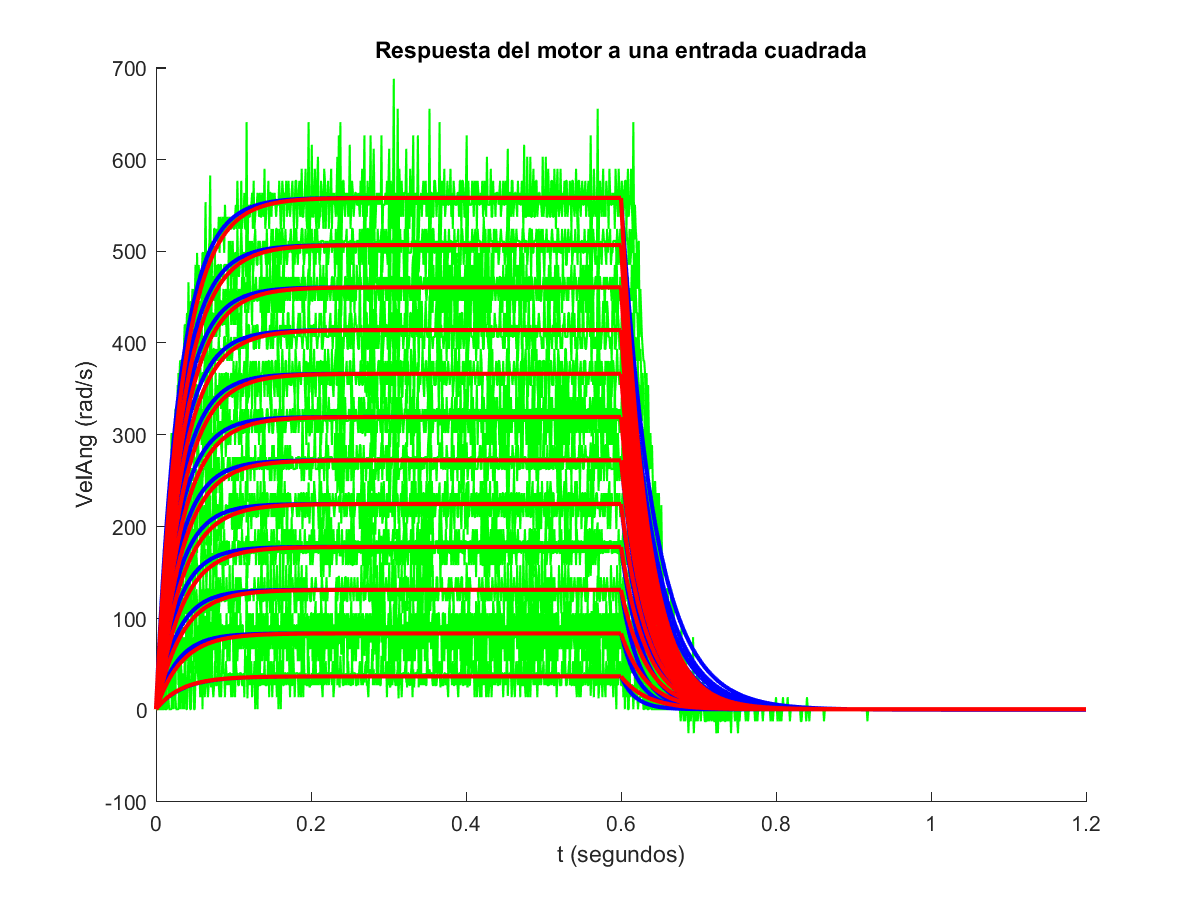
\includegraphics[width=10cm]{vel_ang}
		\caption{Derivada de la posicion (en verde). Ni idea (en rojo). Tampoco (en azul)}
		\label{velAng}
	\end{center}
\end{figure}

La segunda fase consiste en estudiar el régimen transitorio para realizar el cálculo del polo medio y la varianza mínima para cada valor de tensión.
En la figura \ref{polos} se pueden apreciar los 12 polos obtenidos, cuya combinación lineal explicada en la sección 3.2.2. del documento de modelado\cite{modelado}
da como resultado un polo $pM=29.9483$.

Cuando se considera el motor en régimen permanente la función de transferencia queda como:

\begin{equation}
	\label{eq:trans0}
	\dot{\theta}_m (0) = K/p
\end{equation}

A partir de la zona en la que se considera terminado el régimen transitorio se obtiene el valor de la velocidad nominal del motor para cada valor de tensión.
Usando estos valores junto el valor del polo obtenido anteriormente se puede aplicar la ecuación \ref{eq:trans0} pueden obtener los valores de ganancia $K$ indicados en la
figura \ref{valoresK}.
Usando estos valores se obtiene la ganancia media $KM=1372.1456$ y las tensiones de entrada equivalente de la tabla \ref{veq}.

\begin{figure}[htbp]
	\begin{center}
		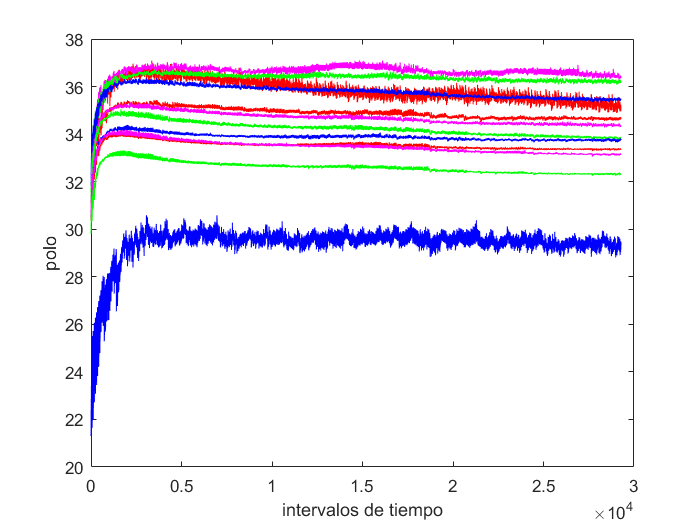
\includegraphics[width=10cm]{polos}
		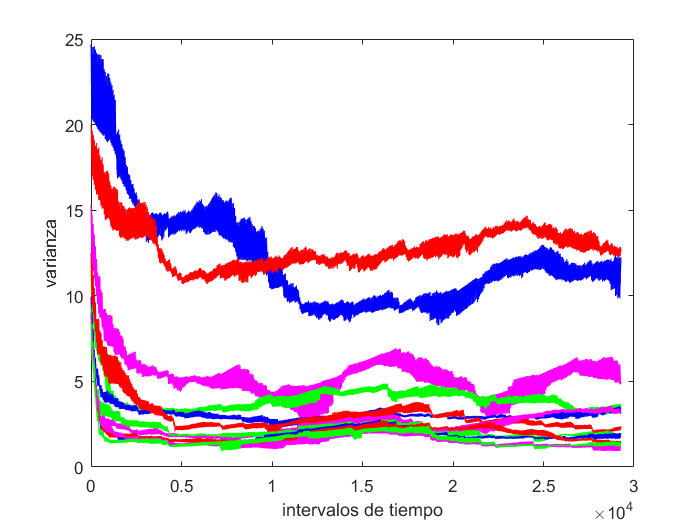
\includegraphics[width=10cm]{varianza}
	\end{center}
	\caption{}
	\label{polos}
\end{figure}

\begin{figure}[htbp]
	\begin{center}
		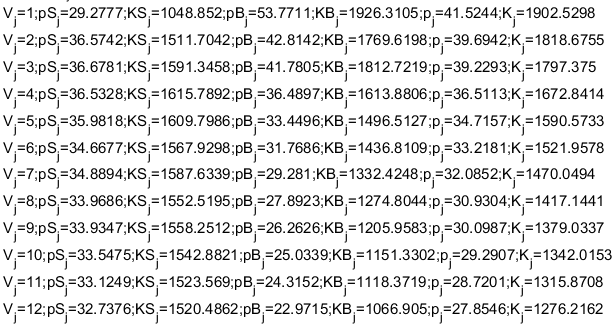
\includegraphics[width=10cm]{valores_fase_3}
		\caption{Valores obtenidos en la fase 3}
		\label{valoresK}
	\end{center}
\end{figure}

\begin{table}[hbt]
	\begin{center}
		\begin{tabular}{c c}
			Tensión de entrada($V$) & Tensión equivalente($V$) \\
			\hline
			1 & 0,7818964 \\
			2 & 1,8042383 \\
			3 & 2,8408659 \\
			4 & 3,8612983 \\
			5 & 4,8823767 \\
			6 & 5,9227804 \\
			7 & 6,9522867 \\
			8 & 7,9803429 \\
			9 & 9,0200431 \\
			10 & 10,037934 \\
			11 & 11,042630 \\
			12 & 12,164355 \\
			\end{tabular}
	\end{center}
	\caption{Valores de tensión equivalentes calculados}
	\label{veq}
\end{table}

También se ha calculado el error cuadrático que es $J=0.0918$. De las figuras se pueden obtener los valores del polinomio impar de grado 12 que están representados en la figura \ref{polinomioA}
También se calcula el polinomio inverso, que serán necesario para el siguiente apartado.

\begin{figure}[htbp]
	\begin{center}
		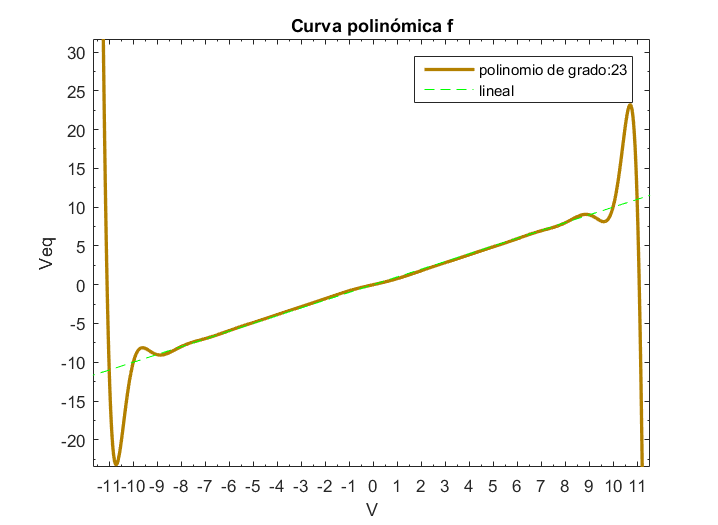
\includegraphics[width=10cm]{curva_polinomica}
		\caption{}
		\label{polinomioA}
	\end{center}
\end{figure}

\begin{equation}
a =
\left( \begin{array}{c}
a_1 \\
a_3 \\
\vdots \\
a_23
\end{array} \right)
=
\left( \begin{array}{c}
0,701961209032454  \\
0,0945362588079597  \\
-0,0160613536061577  \\
0,00154761933773519  \\
-9,05842600897708 \times 10^{-5}  \\
3,36970267186654\times 10^{-6}  \\
-8,16569483050979\times 10^{-8}  \\
1,29780689392616\times 10^{-9}  \\
-1,33533762669408\times 10^{-11}  \\
8,52938300661312\times 10^{-14}  \\
-3,06295258196779\times 10^{-16}  \\
4,71095903040637\times 10^{-19}
\end{array} \right)
\end{equation}

Finalmente, sustituyendo los valores obtenidos anteriormente en la ecuación \ref{eq:trans} se obtiene:

\begin{equation}
	\label{eq:transVal}
	\dot{\theta}_m (s) = \frac{1372.1456}{s+29.9483}
\end{equation}


\subsection{Problemas encontrados durante la obtención de las gráficas de esta sección}
Como el profesor podrá recordar, nuestro grupo tuvo ciertos problemas a la hora de obtener las gráficas presentadas en esta sección, concretamente las gráficas de polos y de varianza,
ya que estas aparecían con intervalos en blanco sin saber muy bien la razón. Tras indagar sobre el tema, se encontró cual era la causa
del problema y se solucionó. Parece ser que la interrupción que se había activado para el control del tiempo por milisegundos a veces
no era lo bastante rápida ya que la interrupción encargada de tomar datos en los flancos de subida o bajada de los pines de los que obtenemos
los datos de movimiento del motor parecía ser más rápida, por lo que tomaba dos datos con el mismo tiempo, por lo que al calcular la velocidad se obtenían infinitos.
Para solucionar este contratiempo, se ha realizado una media de los tiempos junto con la media de los datos de tensión.
Esta modificación del software realizado en matlab se encuentra en el repositorio GitHub.

También tuvimos ciertos problemas con la activación de las interrupciones generadas por \emph{timers} comentadas en la sección \ref{int}, ya que la nomenclatura usada en el \emph{framework} no es nada clara.
Al parecer, en el driver que controla los timers se considera que existen únicamente 3 (TC0, TC1 y TC2) con 3 canales cada uno que se seleccionan con un parámetro en sus funciones,
sin embargo, tanto el el driver del PCM como en controlador de las interrupciones (NVIC), existen 9 timers (TC0, TC1, ..., TC8) completamente independientes. Por lo que era necesario
usar distintas referencias según el driver con el que estuvieras interactuando. Todo esto fue encontrado en el apartado 7.1 del datasheet del microprocesador \cite{SAM3X/A}

\section{Análisis, diseño e implementación de un controlador P para un control de posición angular \label{control}}

Para implementar un controlador de la posición es suficiente con hacer un bucle de realimentación lineal,
sin embargo, para que sea más eficaz, se ha usado el modelo del motor que se ha obtenido en la sección anterior.

Se ha usado el cálculo del voltaje equivalente para obtener los valores de tensión real que hay que introducir al motor para que se comporte de la forma esperada por el
controlador lineal.

Para ello se ha usado la inversa de la función no lineal para el modelo del motor, representada en la figura \ref{polinomioB} y sus coeficientes son:

\begin{equation}
b =
\left( \begin{array}{c}
b_1 \\
b_2 \\
\vdots \\
b_12
\end{array} \right)
=
\left( \begin{array}{c}
1,35449294076669 \\
-0,139208967806144 \\
0,0272672229765444 \\
-0,00288932286118707 \\
0,000180442706051049 \\
-7,01927496494115\times 10^{-6} \\
1,75435087512626\times 10^{-7} \\
-2,84770776397949\times 10^{-9} \\
2,97085236393373\times 10^{-11} \\
-1,91325972520681\times 10^{-13} \\
6,89609494470547\times 10^{-16} \\
-1,06057220426799\times 10^{-18}

\end{array} \right)
\end{equation}

\begin{figure}[htbp]
	\begin{center}
		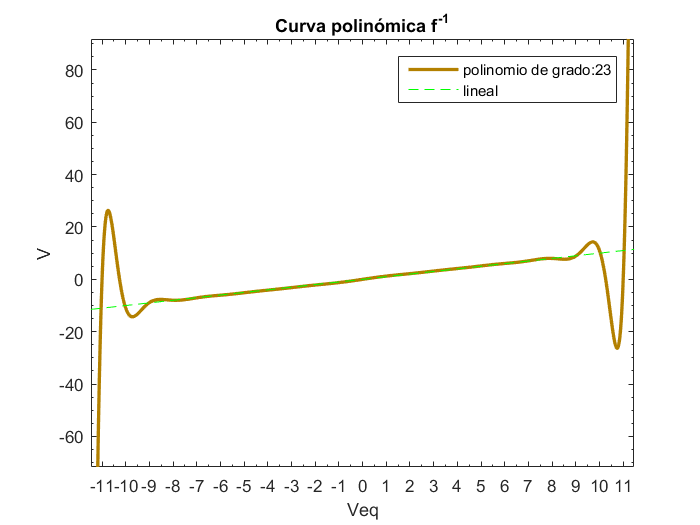
\includegraphics[width=10cm]{curva_polinomica_inversa}
		\caption{}
		\label{polinomioB}
	\end{center}
\end{figure}

Dado que estamos trabajando con un microprocesador de baja potencia no se ha implementado la función matemática en software, si no que se ha usado una \emph{lookup table} generada
en Matlab de la que el controlador obtiene los valores oportunos.

Debido a que la última parte de la función era muy irregular, se ha decidido linealizar los valores a partir del cual estos cambiaban de forma demasiado brusca. Para conseguir los valores
que se utilizan en el código se creado un script en matlab. Se vuelve a remitir al repositorio de GitHub \cite{git} donde se encuentra dicho código.

\section{Conclusiones}
En este trabajo se ha modelado un motor de corriente continua con el uso de varios recursos que se nos han proporcionado, y con el seguimiento de la documentación de la asignatura. Aquí se han presentado los
resultados de este modelado, que en principio consideramos satisfactorios, esperando haber cumplido los objetivos del mismo.

Hemos tenido una gran carga de investigación ya que hemos tenido que utilizar recursos y funciones con los que no estábamos muy familiarizados. Esto ha requerido tiempo, ya que nos hemos
encontrado con varios errores y problemas que no esperábamos pero que por suerte hemos conseguido solventar. Por esto mismo, consideramos que esta es la parte que más valor nos va a aportar de
este trabajo.


\begin{thebibliography}{9}
\bibitem{git} \href{https://github.com/jjalberca/reallabo2018}{Repositorio del proyecto alojado en GitHub}
\bibitem{modelado} Félix Monasterio-Huelin y Álvaro Gutiérrez: \href{http://robolabo.etsit.upm.es/asignaturas/seco/apuntes/modelado.pdf}{Modelado de un motor DC}
\bibitem{SAM3X/A} Atmel Corporation \href{http://ww1.microchip.com/downloads/en/DeviceDoc/Atmel-11057-32-bit-Cortex-M3-Microcontroller-SAM3X-SAM3A_Datasheet.pdf}{Datasheet SAM3X / SAM3A Series}
\bibitem{framework} Atmel Corporation \href{http://asf.atmel.com/docs/latest/search.html?device=sam3x}{Atmel Software Framework}
\end{thebibliography}


\end{document}
